\documentclass[11pt,pdftex,portrait,letterpaper]{article}
\usepackage[hdivide={1in,*,1in},
            vdivide={1in,*,1in},
%            showframe
            ]{geometry}

\usepackage{graphicx}
\usepackage{longtable}
\usepackage{acronym}
\usepackage{verbatim}
\usepackage{subfigure}
\usepackage{fancyhdr}
\pagestyle{fancy}
\usepackage{listings}
\usepackage{color}
\usepackage{lastpage}
\usepackage{amsmath}
\usepackage{amssymb}
\usepackage{gensymb}
\usepackage{tabularx}
\usepackage[backend=biber, style=ieee]{biblatex}
\addbibresource{references.bib}

% Default margins are too wide all the way around. Reset them here
\setlength{\topmargin}{-.5in}
\setlength{\textheight}{9in}
\setlength{\oddsidemargin}{.125in}
\setlength{\textwidth}{6.25in}

\lhead{ECEN 935}
\chead{}
\rhead{\thepage\ of \pageref{LastPage}}
%\lfoot{\hline}
\lfoot{}
\cfoot{\small{University of Nebraska - Lincoln Department of Electrical Engineering}}
\rfoot{}
\renewcommand{\footrulewidth}{0.5pt}

\lstset{
  language=Matlab,        % specify the language
  basicstyle=\ttfamily\scriptsize,   % font style for the code
  keywordstyle=\color{blue}, % keywords in blue
  commentstyle=\color{green}, % comments in green
  stringstyle=\color{red}, % strings in red
  numbers=left,           % display line numbers on the left
  numberstyle=\tiny,      % style for the line numbers
  stepnumber=1,           % line numbers step
  frame=single,           % add a frame around the code
  breaklines=true         % allow line breaks
}

\begin{document}

\vspace*{30ex}
\begin{center}

\textbf{Feed-forward Artificial Neural Network (ANN) and Backpropagation in Matlab}\\

\vspace{4ex}
Computational Intelligence - University of Nebraska \\

\vspace{4ex}
Zachary Swanson\\
September 27, 2024\\

\end{center}


\pagebreak
\tableofcontents
%\pagebreak
%\listoffigures
%\addcontentsline{toc}{section}{{\bf List of Figures}}
\pagebreak


\section{Abstract}

This experiment explores the implementation of a Multilayer Perceptron (MLP) to fit the function $y=2x^2+1$, examining the effects of learning gain, momentum gain, and neuron quantity in the hidden layer. Using gradient descent and backpropagation, the model was trained over 10,000 epochs across a range of learning and momentum gain combinations. Results showed that a learning gain of 0.1 and low momentum values achieved the best training performance, minimizing mean-square error (MSE) on both training and test data. However, reducing the learning rate to 0.01 produced similar training performance but improved performance on the test set. The effects of the momentum gain were less obvious.

The impact of hidden layer neuron quantity was also evaluated, revealing a balance between model complexity and convergence speed. At least five neurons were required in the hidden layer to adequately fit the function and increasing the number of neurons improved training and test performance up to 15 neurons. More than 15 neurons improved training performance but negatively impacted test performance. This demonstrates that larger models (i.e. more hidden layer neurons) overfit the training data and did not generalize as well to new data. Overall, the experiment successfully illustrates the core principles of MLP training and the effects of key hyperparameters on performance.

\section[Introduction]{Introduction\footnote{Information condensed and generalized from \cite{qiao2024artificial}, \cite{engelbrecht2007computational}, and \cite{bishop2006pattern}.}}
\subsection{Artificial Neural Networks}
Artificial Neural Networks (ANNs) are a computational model inspired by the biological structure of the brain. They consist of layers of neurons, where each neuron receives inputs, computes a weighted sum of the inputs, adds a bias, and applies a nonlinear activation function to determine its output. The main components of a neuron are:
\begin{itemize}
    \item \textbf{Weights:} The adjustable parameters that determine the influence of each input on the neuron's output.
    \item \textbf{Bias:} A constant added to the weighted sum, providing flexibility in shifting the activation function.
    \item \textbf{Activation Function:} A nonlinear function (e.g., Sigmoid, ReLU, or hyperbolic tangent (tanh)) that introduces non-linearity into the model, enabling it to learn complex patterns.
\end{itemize}

Figure \ref{fig:neuron_mlp} illustrates both an individual neuron (left side) and a multilayer perceptron (MLP) (right side). The artificial neuron graphically demonstrates the main components described above. The inputs are weighted (green boxes) and all the weighted inputs are summed with an additional bias (blue box). The summed value is then passed to the activation function (red circle). The output of the activation function is the output neuron, y. This may be written in a succinct, mathematical representation as

\begin{equation} \label{eq:neuron}
    y = f\left(\left(\sum_{i=1}^{n} w_i \cdot x_i\right) + b\right).
\end{equation}

\begin{figure}[h]
    \centering
    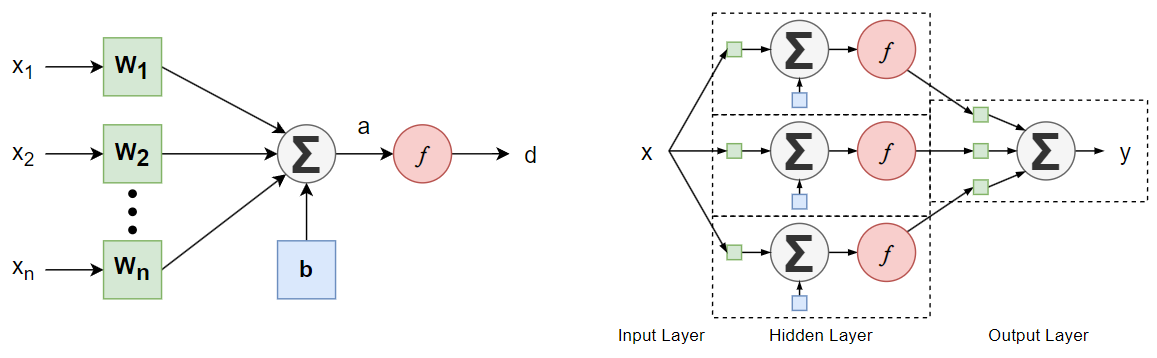
\includegraphics[width=\textwidth]{./figures/neuron_and_mlp}
    \caption{A diagram showing an artificial neuron (left) and a multilayer perceptron (right).}
    \label{fig:neuron_mlp}
\end{figure}

Neural networks typically consist of an input layer, one or more hidden layers, and an output layer. This structure forms a Multilayer Perceptron (MLP), where each layer's outputs become the next layer's inputs. MLPs can learn highly complex functions by stacking multiple layers of neurons. The example provided in Figure \ref{fig:neuron_mlp} has a one input, a single hidden layer with three neurons, and a single output. This example was provided strategically as it resembles the MLP used for function fitting in this assignment. It is important to note that the output layer in Figure \ref{fig:neuron_mlp} does not include an activation function because the goal is to perform regression and achieve a continuous output value. However, for tasks like classification, it may be necessary to include an appropriate activation function (e.g. softmax).

\subsection{Gradient Descent and Backpropagation} \label{sec:gdBackprop}
Gradient descent is an optimization algorithm used to minimize the loss function in machine learning models, including artificial neural networks. The algorithm iteratively updates the model's parameters (weights and biases) in the direction of the steepest descent, as determined by the negative gradient of the loss function. The update rule for the parameters can be expressed mathematically as:
\begin{equation} \label{eq:gd}
    \theta \leftarrow \theta - \eta \nabla L(\theta)
\end{equation}
where \( \theta \) represents the model parameters, \( \eta \) is the learning rate, and \( \nabla L(\theta) \) is the gradient of the loss function with respect to the parameters. The choice of learning rate is crucial, as it determines the step size of each update; a learning rate that is too high can cause the optimization process to diverge, while one that is too low may result in a slow convergence.

An enhancement to the basic gradient descent algorithm is the concept of momentum. Momentum introduces a term that accumulates the past gradients to dampen oscillations and accelerate convergence in the relevant direction. The updated parameter with momentum is given by:
\begin{equation} \label{eq:velocity}
    v_t = \beta v_{t-1} + (1 - \beta) \nabla L(\theta)
\end{equation}
\begin{equation} \label{eq:gdMomentum}
    \theta \leftarrow \theta - \eta v_t
\end{equation}
where \( v_t \) is the velocity, \( \beta \) is the momentum coefficient (typically between 0 and 1), and \( t \) denotes the iteration step. This technique helps in navigating ravines and flat areas of the loss landscape more effectively, ultimately improving the optimization process.

The backpropagation algorithm relies heavily on the chain rule of calculus, which is crucial for efficiently computing gradients in a multi-layered neural network. The chain rule allows for the decomposition of the gradient of the loss function into a product of derivatives of the functions at each layer. This is mathematically expressed as:

\begin{equation} \label{eq:chainrule}
    \frac{\partial L}{\partial \theta} = \frac{\partial L}{\partial \hat{y}} \cdot \frac{\partial \hat{y}}{\partial z} \cdot \frac{\partial z}{\partial \theta}
\end{equation}
where \( \hat{y} \) is the output of the neural network, \( z \) is the intermediate layer's output, and \( L \) is the loss function. By applying the chain rule iteratively through each layer, backpropagation efficiently propagates the error backward, enabling the computation of gradients necessary for the parameter updates. This systematic approach is what allows neural networks to learn complex functions effectively.

\section{Methodology}

The goal of this experiment was to implement a MLP and train it to fit the function 
\begin{equation} \label{eq:targetFn}
    y=2x^2+1.
\end{equation}
Additionally, the experiment seeks to explore the effect of the learning gain and momentum gain on training the model and the effect of neuron quantity in the hidden layer.

\subsection{Architecture Implementation}

As illustrated in Figure \ref{fig:neuron_mlp}, the network consists of an input layer, one hidden layer, and an output layer with no activation function. The network also has a single input and a single output, x and y in Equation \ref{eq:targetFn}, respectively. Figure \ref{fig:neuron_mlp} depicts three neurons in the hidden layer; however, the number of neurons will be a variable that is explored as part experiment.

It should be noted that the weights of the network are initialized randomly in following best practice to break symmetry of the network. If all weights are initialized identically, then they all perform the same calculation and get updated the same. Thus, the layer operates like a single neuron and this negatively impacts the learning capabilities.

The hidden layer in this experiment utilizes the sigmoid function. This function is given by
\begin{equation}\label{eq:sigmoid}
    \sigma(x) = \frac{1}{1+e^{-x}}.
\end{equation}
A convenient feature of this function is that it's derivative may be defined in terms of the function itself. This is useful because the output of the activation function is obtained on the forward pass through the network and may then be used in backpropagation.. The derivative is given by
\begin{equation}\label{eq:sigmoidDeriv}
    \sigma'(x)=\sigma(x) \left(1-\sigma(x)\right)
\end{equation}

Backpropagation was implemented with respect to the equations provided in \cite{qiao2024artificial}. To start, output error was estimated using the sum-squared of the error vector. That is
\begin{equation}
    E=\frac{1}{2}||\underline{e}_y||^2=\frac{1}{2}||\underline{y}-\underline{\hat{y}}||^2
\end{equation}
For conciseness, not all details are provided from \cite{qiao2024artificial} for the following. The error is propagated through the layers to provide a decision error and an activation error. These are given by
\begin{equation}\label{eq:decisionError}
    \underline{e}_d=-V^T\underline{e}_y
\end{equation}
and
\begin{equation}\label{eq:activationError}
    e_{ai}=d_i(1-d_i)e_{di},
\end{equation}
respectively, where $V$ is the vector of output layer weights, $d$ is the vector of outputs from the hidden layer's activation functions and $a$ is the vector of summed weights and biases of the hidden layer neurons (prior to activation). Note that the $d_i(1-d_i)$ term in Equation \ref{eq:activationError} is a result of computing the derivative of the sigmoid activation function as described in Equation \ref{eq:sigmoidDeriv}. Further propagation, results in the following weight update formulas
\begin{equation}
    \Delta V(k)=\gamma_g\underline{e}_y(k)\underline{d}^T(k)+\gamma_m\Delta V(k-1)
\end{equation}
and
\begin{equation}
    \Delta W(k)=\gamma_g\underline{e}_a(k)\underline{x}^T(k)+\gamma_m\Delta W(k-1),
\end{equation}
for the output and hidden layer weights, respectively, where $\gamma_g$ is the learning gain, $\gamma_m$ is the momentum gain, respectively, $x$ is the network inputs, and $W$ is the hidden layer weights. Note that the learning and momentum gain symbols are different here than the  conventional ones used in Section \ref{sec:gdBackprop}. These equations were implemented in Matlab as part of the training method of the MLP class.

\subsection{Matlab Implementation}

The MLP and experiment were implemented in separate Matlab source files to make the code more reusable and easier to manage. Each of the source files may be found in its respective section in the Appendix. Starting from the bottom up, a simple MLP-layer class was implemented (see Section \ref{sec:appMlpLayer}). This class was responsible for storing the weights of a given layer and implementing a $forward(\cdot)$ method that would execute the weighted sum and activation function.

The layer class was then used within an overarching MLP class (see Section \ref{sec:appMLP}) where a hidden layer and an output layer were instantiated. The MLP class implemented a $forward(\cdot)$ class that sequentially executed the $forward(\cdot)$ methods of the layer classes. The MLP class also implemented a $training(\cdot)$ method that required input data and expected labels. For each datum the method performed a forward pass on the datum, computed the loss with provided label, performed backpropagation, and updated the weights accordingly. 

Lastly, a main Matlab script (see Section \ref{sec:appMain}) implemented the full experiment. This included generating data for the function $y=2x^2+1$, splitting it into training and test sets, and instantiating an MLP object. The MLP object was then trained for multiple epochs and the main script then recorded and plotted the necessary results.
 
\subsection{Training and Evaluation} \label{sec:trainEval}

A dataset was generated using Equation \ref{eq:targetFn} with x ranging from -1 to 1 in 0.01 increments. This resulted in 201 values. The data was split into training and test sets with an 80-20 split. This was achieved by randomly shuffling the indices and selecting 20\% for the test set.

For each phase of the experiment the model was trained for 10,000 epochs on the training data, where an epoch represented training the model on all data in the training set. The mean-square error was recorded after each epoch and used to generate a MSE-vs-epoch plot. After training for 10,000 epochs, the model was evaluated on the unseen test set. The MSE for the test set was recorded and a plot of the test predictions versus the actual function was generated.

The training and evaluation were repeated for 54 combinations of learning gains and momentum gains with five neurons in the hidden layer. These combinations were based on the sets [0.01, 0.1, 0.5, 0.7, 0.9,  1] and [0, 0.0001, 0.001, 0.01, 0.1, 0.5, 0.7, 0.9, 1] for learning gain and momentum gain, respectively. After evaluating all combinations, the optimal learning and momentum gain were selected and evaluated for the following set of neurons in the hidden layer, [3, 4, 6, 7, 8, 9, 10, 15, 20, 25, 30, 50, 100].

\section{Results}

Table \ref{t:gainCombos} presents the results of the top-20 combinations of learning and momentum gains ranked by the average MSE for the training data. Learning gain of $\gamma_g=0.1$ performed best in terms of minimum and average MSE on the training data across a range of momentum gains. This top average and minimum MSE performance were achieved with lower values for momentum gain, i.e. $\gamma_m \leq 0.1$. Continuing in terms of minimum and average training MSE, a smaller learning gain of $\gamma_g=0.01$ achieved the next best performance across a range of momentum gains. As expected, the higher learning rate achieved faster convergence. However, the effects of the momentum gain on convergence were less obvious.

\begin{table}[h]
\label{t:gainCombos}
\centering
\begin{tabular}{|c|c|c|c|c|c|c|c|}
\hline
\textbf{n} & \textbf{$\gamma_g$} & \textbf{$\gamma_m$} & \textbf{Min MSE} & \textbf{Avg MSE} & \textbf{Test MSE} & \textbf{Conv.} & \textbf{Slow} \\ 
\hline
5  & 0.1  & 0.1   & 0.00039783 & 0.00095322 & 0.0040762  & 500  & 3000  \\ 
5  & 0.1  & 0.01  & 0.00037262 & 0.00104102 & 0.00376093 & 500  & 3000  \\ 
5  & 0.1  & 0.001 & 0.00037084 & 0.00106526 & 0.00373522 & 500  & 3000  \\ 
5  & 0.1  & 0.0001& 0.00037067 & 0.00106809 & 0.00373269 & 500  & 3000  \\ 
5  & 0.1  & 0     & 0.00037065 & 0.00106841 & 0.00373241 & 500  & 3000  \\ 
5  & 0.01 & 0.7   & 0.00101952 & 0.00356875 & 0.00295116 & 500  & 3000  \\ 
5  & 0.01 & 0.5   & 0.00096068 & 0.00438433 & 0.00236396 & 750  & 4000  \\ 
\textbf{5}  & \textbf{0.01} & \textbf{0.1}  & \textbf{0.00128718} & \textbf{0.00654138} & \textbf{0.00211061} & \textbf{1000} & \textbf{6000} \\ 
5  & 0.01 & 0.01  & 0.00136564 & 0.00707284 & 0.00210789 & 1000 & 6000  \\
5  & 0.01 & 0.001 & 0.00137338 & 0.00712676 & 0.00210833 & 1000 & 6000  \\ 
5  & 0.01 & 0.0001& 0.00137415 & 0.00713216 & 0.00210838 & 1000 & 6000  \\ 
5  & 0.01 & 0     & 0.00137424 & 0.00713276 & 0.00210838 & 1000 & 6000  \\ 
5  & 0.1  & 0.5   & 0.00324193 & 0.02800445 & 0.86249161 & 1000 & 4000  \\ 
5  & 0.01 & 0.9   & 0.01344485 & 0.02924594 & 0.04370383 & 1500 & 2000  \\ 
5  & 0.5  & 0.1   & 0.00125328 & 0.0293106  & 0.5049517  & 1750 & 2000  \\ 
5  & 0.5  & 0.01  & 0.00130659 & 0.04092462 & 0.55857029 & 1000 & 4000  \\ 
5  & 0.5  & 0.001 & 0.0013151  & 0.04769672 & 0.48489041 & 1000 & 4000  \\ 
5  & 0.5  & 0.0001& 0.00131599 & 0.04894962 & 0.47487551 & 1000 & 4000  \\ 
5  & 0.5  & 0     & 0.00131609 & 0.04909892 & 0.4737155  & 3500 & 6000  \\ 
5  & 0.5  & 0.5   & 0.00127123 & 0.05070485 & 0.75981172 & 1750 & 2000  \\ 
\hline
\end{tabular}
\caption{Comparison of MSE values, convergence (Conv), and slow down (Slow) epochs for top 20 learning gain ($\gamma_g$) and momentum gain ($\gamma_m$) combinations ranked by average training MSE. Selected optimal combination shown in bold.}
\end{table}

For selecting optimal learning and momentum gains, the evaluation was extended to include the MSE on the test set that was withheld during training. This provides a better sense of how well the model generalizes to new data. As demonstrated in Table \ref{t:gainCombos}, the top-five minimum and average training MSE using $\gamma_g=0.1$ exhibited a higher test MSE than the following five results using $\gamma_g=0.01$. The optimal learning and momentum gain combination, $\gamma_g=0.01$ and $\gamma_m=0.1$, are shown in bold text in Table \ref{t:gainCombos}. This combination was selected because it seemed to provide the best trade-off between training performance and generalizing to the test set when compared to the other results. Furthermore, this combination was used for part B of the experiment.

Qualitatively, Figure \ref{f:gainsCompare} shows learning curve and function fitness plots for the optimal combination described above (left) and a sub-optimal combination (right) using $\gamma_g=0.5$ and $\gamma_m=0.1$. As demonstrated, the optimal combination on the left shows a stable, characteristic learning curve that rapidly declines initially before settling into the minima. As a result, the training process produces a model that very closely fits the target function. The sub-optimal combination exhibited unstable training which occurs when the learning rate is too high. In such cases, the training process tends to jump back and forth over the minima and generally does not settle to the global minima. In the provided example, the training  appears to settle into some sort of local minima as the learning curve flattens out. However, this is clearly not the global minimum based on the poor fitness of the predictions compared to the target function in the bottom-right of Figure \ref{f:gainsCompare}. Other combinations with higher learning and momentum gains exhibited worse training performance as the gradient exploded, producing greater error with each epoch.

\begin{figure}[h]
    \centering
    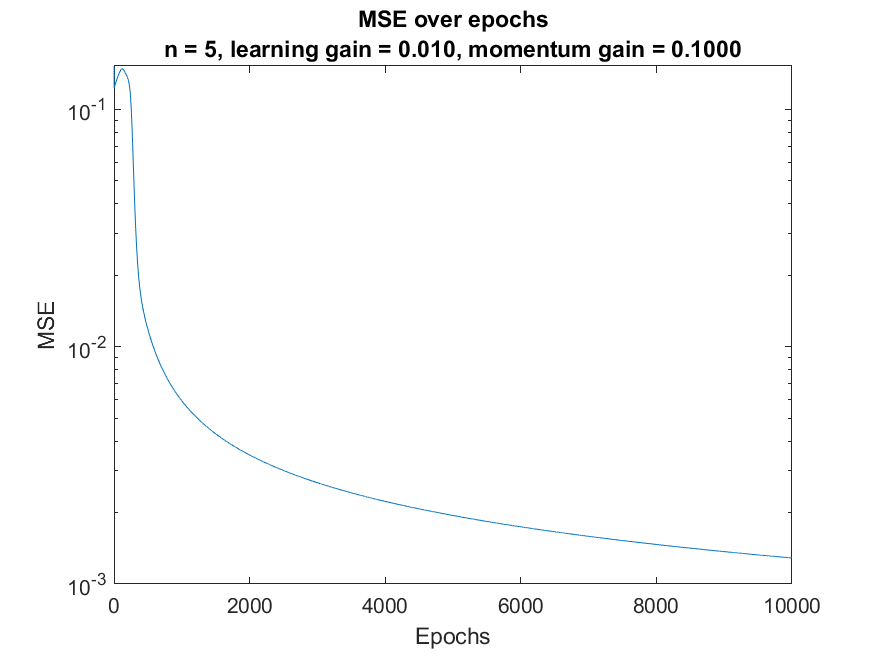
\includegraphics[width=0.45\textwidth]{./figures/mse_5_0.010_0.1000}
    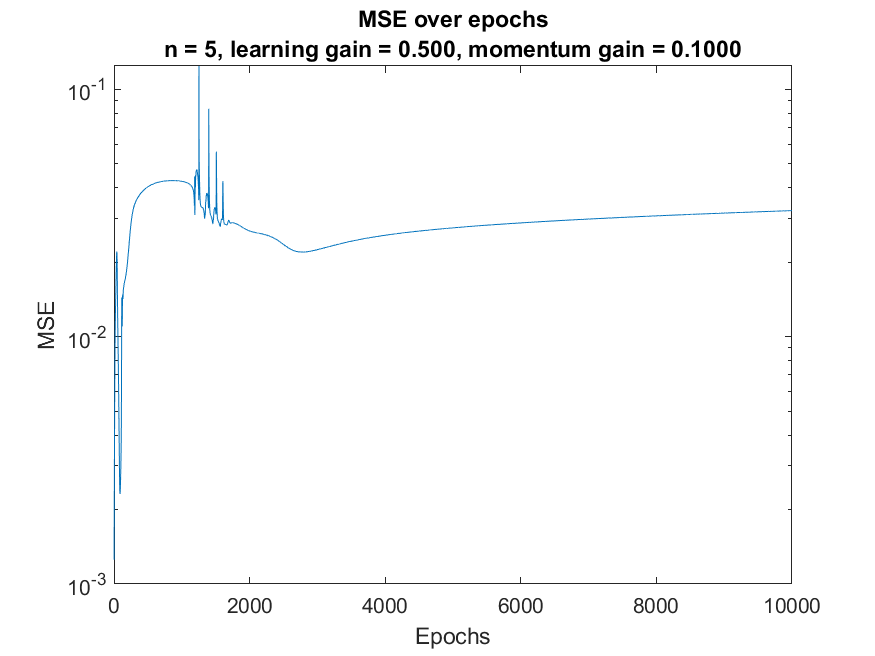
\includegraphics[width=0.45\textwidth]{./figures/mse_5_0.500_0.1000}\\
    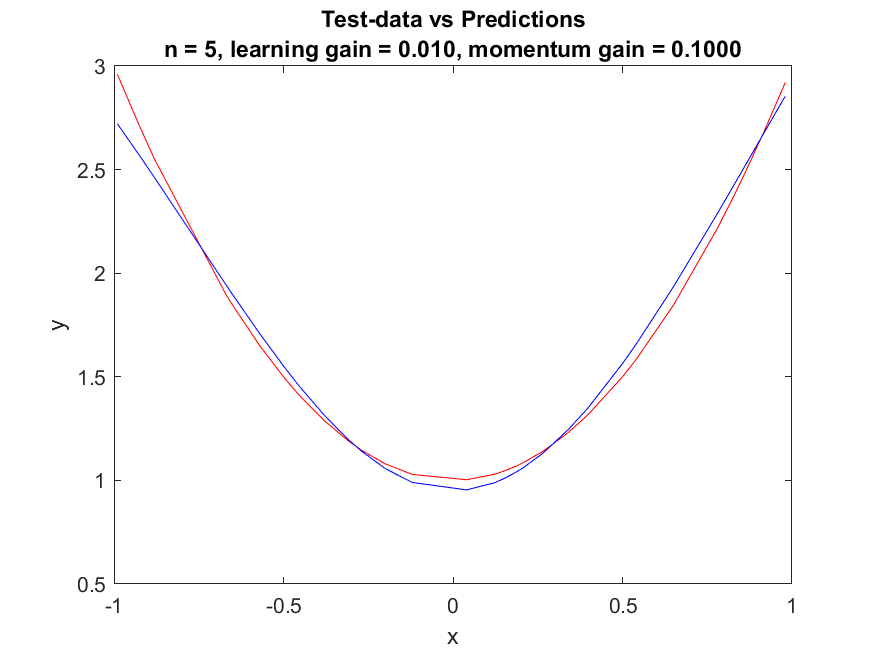
\includegraphics[width=0.45\textwidth]{./figures/function_fitting_5_0.010_0.1000}
    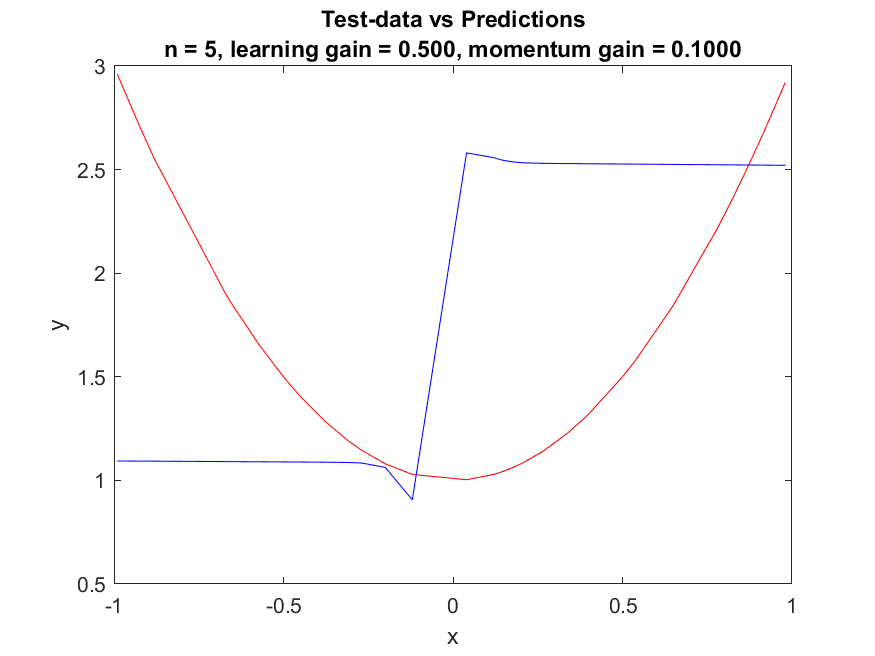
\includegraphics[width=0.45\textwidth]{./figures/function_fitting_5_0.500_0.1000}
    \caption{MSE versus training epochs (top) and predicted (blue) versus actual (red) function curves (bottom) for $\gamma_g=0.01$ (left) and $\gamma_g=0.5$ (right).}
    \label{f:gainsCompare}
\end{figure}

Table \ref{t:nHidden} presents the results of the second part of the experiment that fixed the learning and momentum gains at $\gamma_g=0.01$ and $\gamma_m=0.1$, respectively, varied the number of neurons in the hidden layer ($n$). In terms of convergence, it was expected that the number of epochs required to converge would increase with the number of neurons. This was based on the idea that more neurons means more parameters and more parameters should require more training. This trend was observed for $n=3$ to $n=20$; however for $n={25, 30, 50}$ convergence was achieved significantly faster. It's possible that the random initialization of an increased number of parameters started the training nearer to the minima than it did for the smaller models.

\begin{table}[h]
\label{t:nHidden}
\centering
\begin{tabular}{|c|c|c|c|c|c|c|c|}
\hline
\textbf{n} & \textbf{$\gamma_g$} & \textbf{$\gamma_m$} & \textbf{Min MSE} & \textbf{Avg MSE} & \textbf{Test MSE} & \textbf{Conv.} & \textbf{Slow} \\ 
\hline
3  & 0.01 & 0.1  & 0.14905572 & 0.14938844 & 0.22683948 & 500  & 1500  \\ 
4  & 0.01 & 0.1  & 0.14003208 & 0.14487019 & 0.26046795 & 500  & 1000  \\ 
5  & 0.01 & 0.1  & 0.00128718 & 0.00654138 & 0.00211061 & 1000 & 6000  \\ 
6  & 0.01 & 0.1  & 0.00120851 & 0.00734823 & 0.00200825 & 1000 & 6000  \\ 
7  & 0.01 & 0.1  & 0.00114541 & 0.00533135 & 0.00196022 & 1000 & 6000  \\ 
8  & 0.01 & 0.1  & 0.00101409 & 0.00488077 & 0.00174268 & 1000 & 6000  \\ 
9  & 0.01 & 0.1  & 0.00099606 & 0.00470923 & 0.00183731 & 1000 & 6000  \\ 
10 & 0.01 & 0.1  & 0.00096739 & 0.00684848 & 0.00184934 & 1500 & 8000  \\ 
15 & 0.01 & 0.1  & 0.00069597 & 0.00385866 & 0.00155294 & 1500 & 8000  \\ 
20 & 0.01 & 0.1  & 0.00068213 & 0.0031954  & 0.00182746 & 1500 & 8000  \\ 
25 & 0.01 & 0.1  & 0.00052848 & 0.0029627  & 0.00169468 & 500  & 3000  \\ 
30 & 0.01 & 0.1  & 0.00043896 & 0.00276995 & 0.0016466  & 500  & 3000  \\ 
50 & 0.01 & 0.1  & 0.00036168 & 0.00280803 & 0.0020893  & 1000 & 4000  \\ 
100& 0.01 & 0.1  & 0.0000668  & 0.00295148 & 0.00195905 & 2500 & 4000  \\ 
\hline
\end{tabular}
\caption{Comparison of MSE values, convergence (Conv), and slow down (Slow) epochs for a various number of neurons in the hidden layer ranging from 3 to 100.}
\end{table}

Figure \ref{fig:mse_v_neurons} plots the minimum training MSE, average training MSE, and test MSE results from Table \ref{t:nHidden}. As demonstrated, all three curves show significantly improved performance with increased number of neurons up to six neurons and then the curves flatten out. The 
minimum training MSE (blue) continues to slowly decrease with increased number of neurons, but the test MSE (green) actually begins to increase after 15 neurons. 

\begin{figure}[!h]
    \centering
    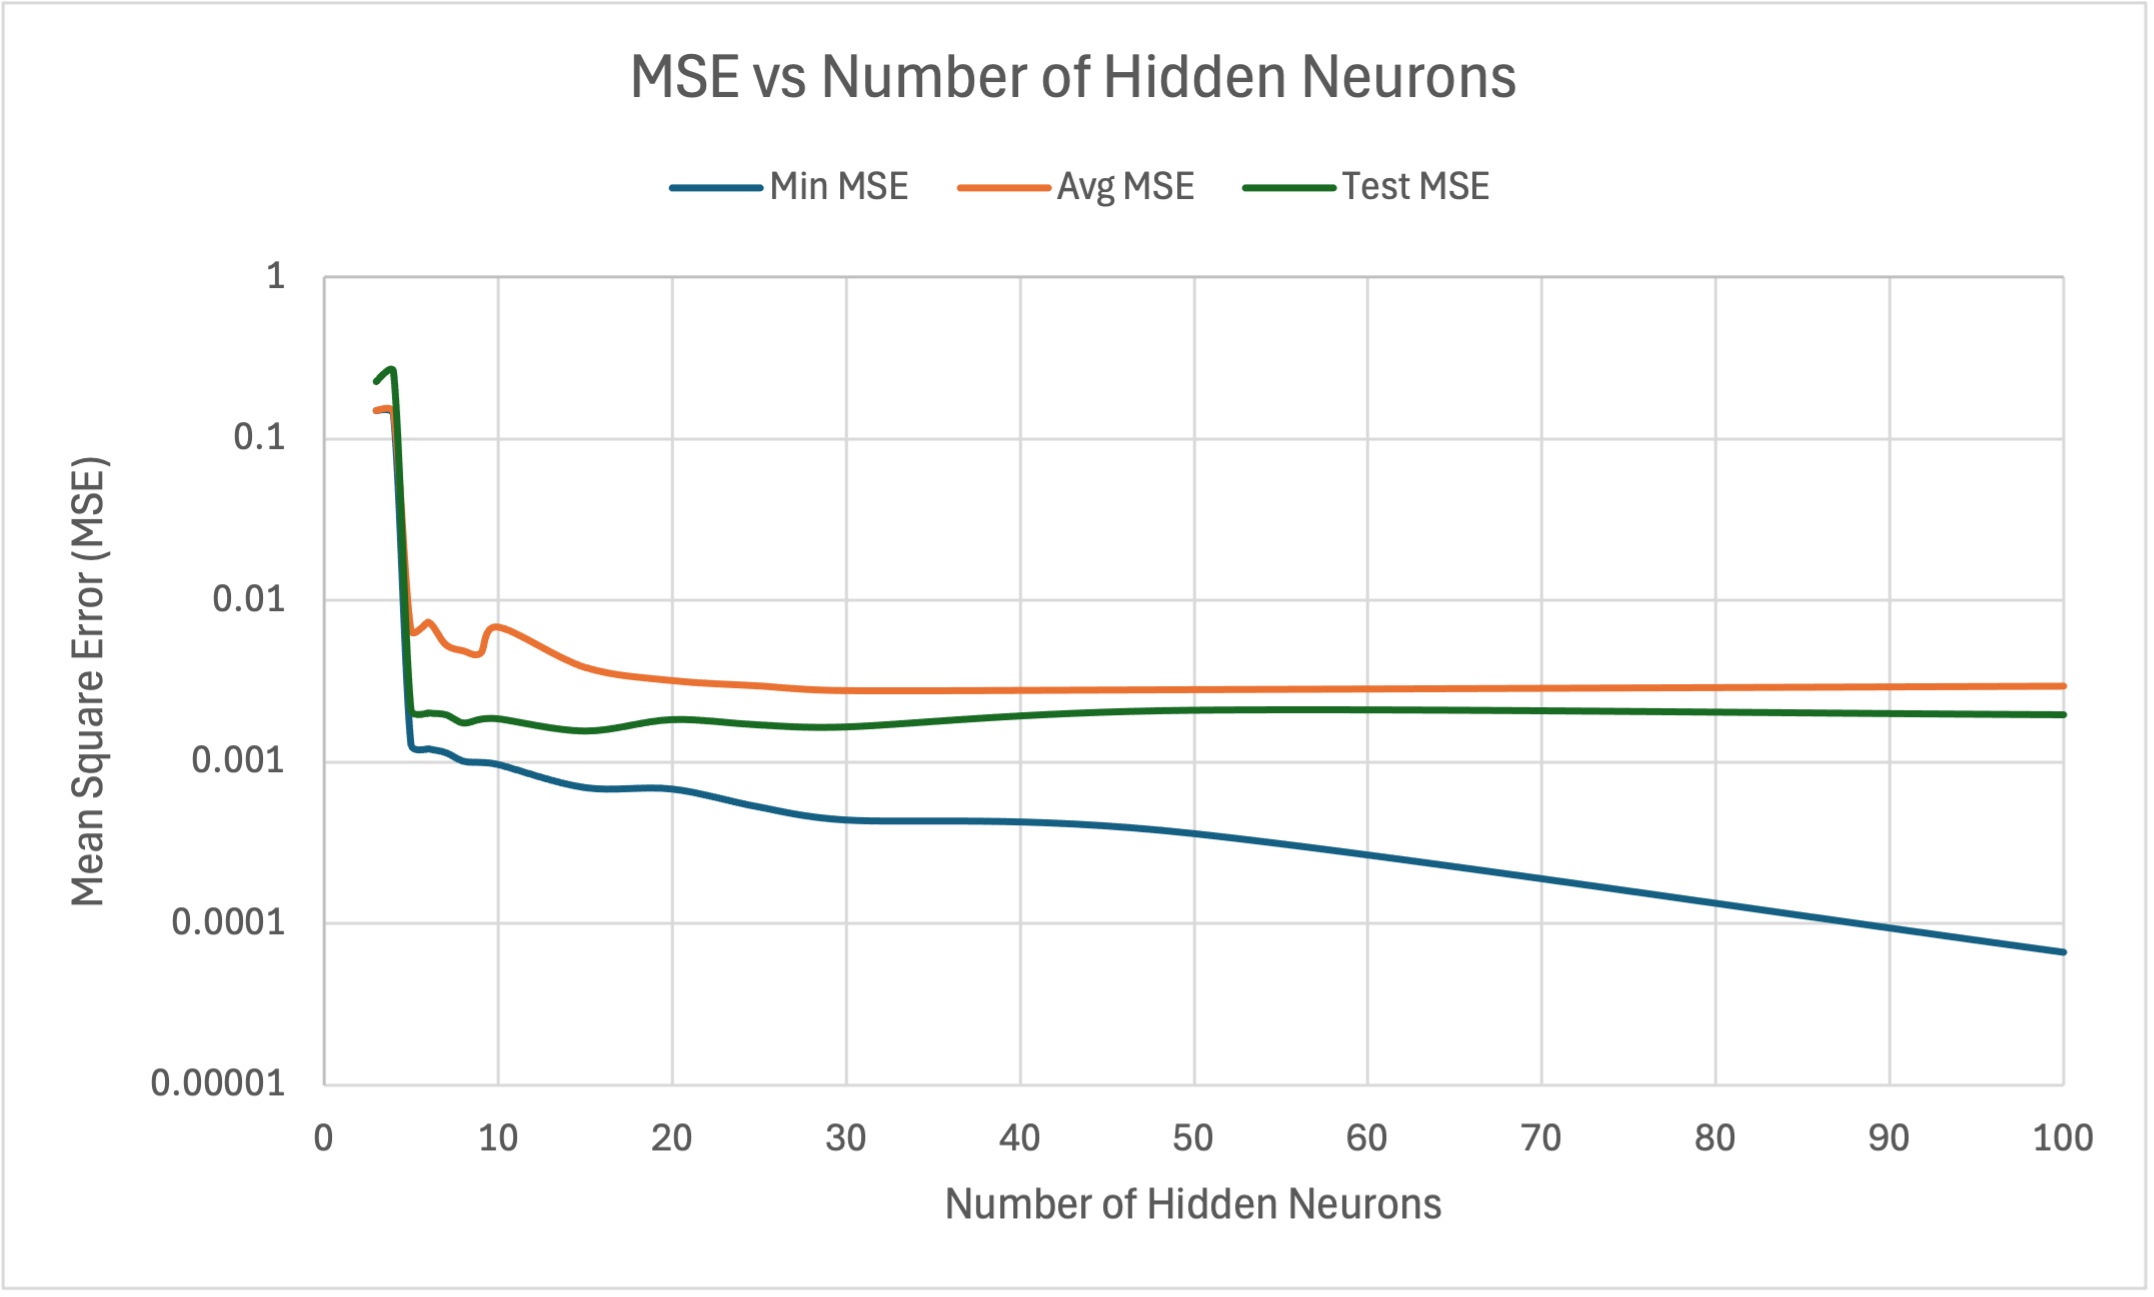
\includegraphics[width=0.85\textwidth]{./figures/mse_v_neurons}
    \caption{A plot of the minimum, average, and test mean-squared errors (MSE) as a function of the number of neurons in the hidden layer.}
    \label{fig:mse_v_neurons}
\end{figure}

The improvement of training performance and decrease testing performance demonstrates the effect of overfitting when a model has too many parameters with respect to the number of training samples. In such cases, larger models will exhibit the best training performance but underperform when presented with new data that the model has not seen before. Given the simplicity of the target, quadratic function (Equation \ref{eq:targetFn}) it was expected that a larger model would overfit. However,  it would be interesting to explore the effects of generating a larger dataset as a future experiment.

Lastly, Figure \ref{f:hiddenCompare} qualitatively demonstrates the difference in learning curves and function fitness for a small number of neurons (left, 3) and a large number of neurons (right, 100) in the hidden layer. These plots may also be compared with the left two plots of Figure \ref{f:gainsCompare} with $\gamma_g=0.01$, $\gamma_m=0.1$, and $n=5$. As discussed above, convergence is achieved quicker for smaller number of neurons, but the MSE at convergence is much greater because the smaller model has converged to a local minima versus the global minima. This is because the smaller model lacks the complexity to fit Equation \ref{eq:targetFn}. This is clearly demonstrated by comparing the function fitness plots in the bottom of Figure \ref{f:hiddenCompare}.

\begin{figure}[h]
    \centering
    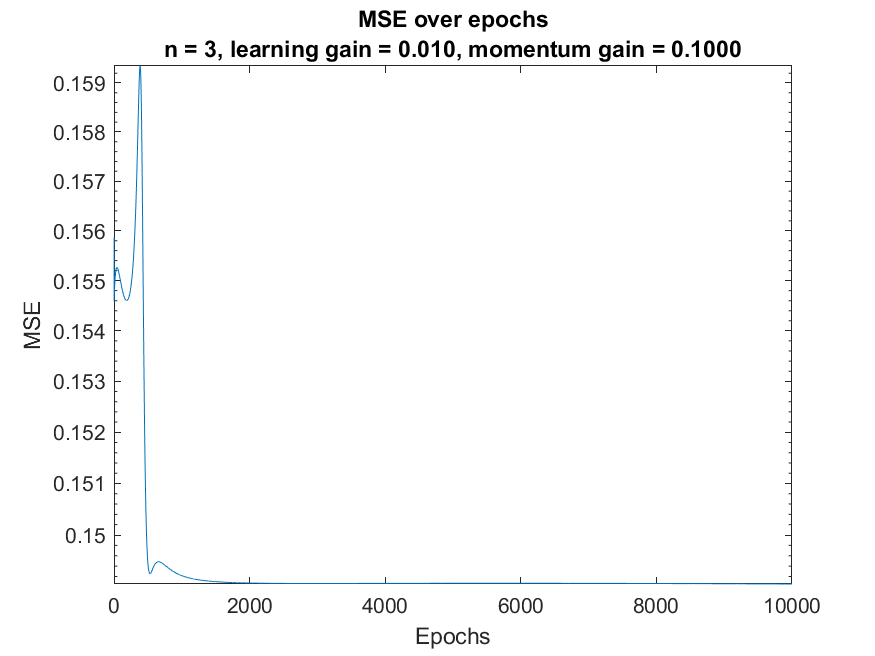
\includegraphics[width=0.48\textwidth]{./figures/mse_3_0.010_0.1000}
    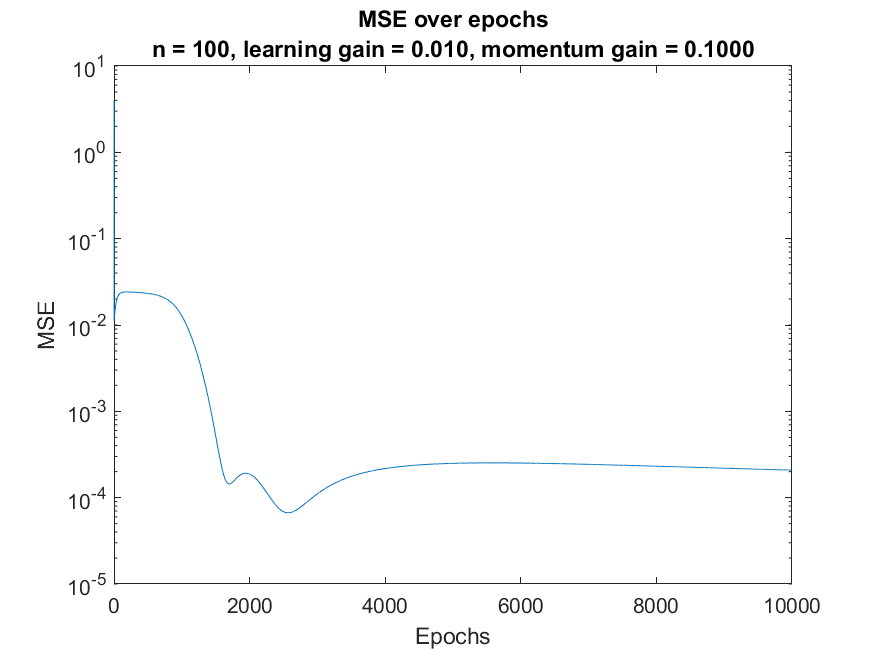
\includegraphics[width=0.48\textwidth]{./figures/mse_100_0.010_0.1000}\\
    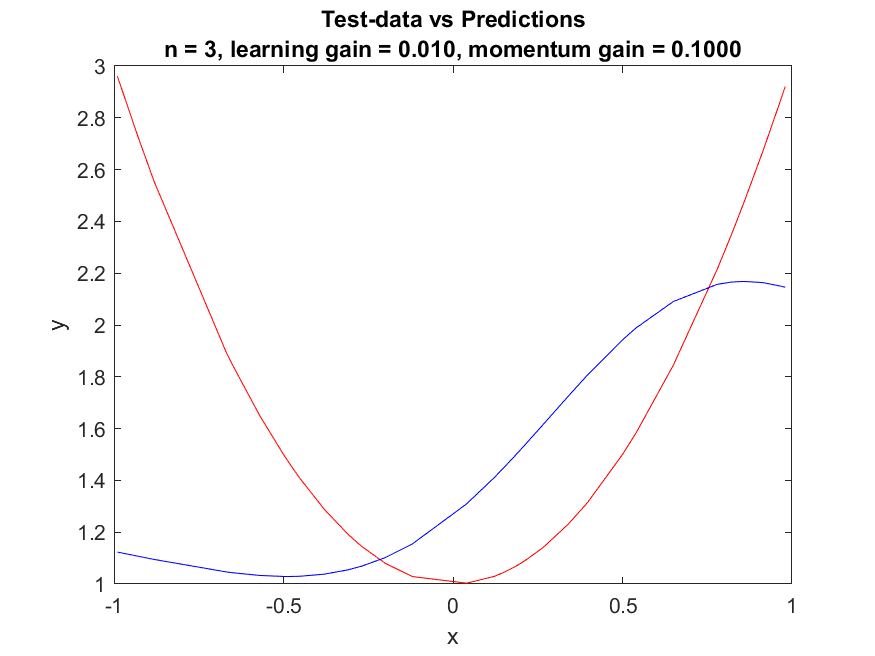
\includegraphics[width=0.48\textwidth]{./figures/function_fitting_3_0.010_0.1000}
    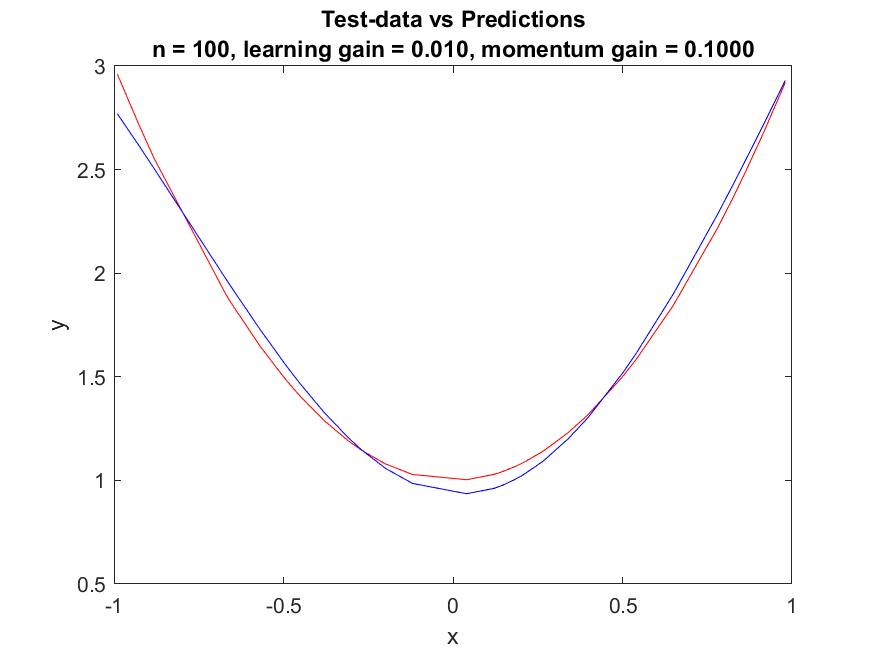
\includegraphics[width=0.48\textwidth]{./figures/function_fitting_100_0.010_0.1000}
    \caption{MSE versus training epochs (top) and predicted (blue) versus actual (red) function curves (bottom) for $\gamma_g=0.01$ (left) and $\gamma_g=0.5$ (right).}
    \label{f:hiddenCompare}
\end{figure}

\section{Conclusion}

The results of this experiment highlight the sensitivity of MLP training to the choice of learning and momentum gains, particularly in the context of fitting a relatively simple quadratic function. Across 54 combinations of these parameters, a learning gain of $\gamma_g=0.1$, $\gamma_m\leq0.1$ consistently yielded the lowest average and minimum MSE on the training data. This combination also demonstrated stable convergence within 3000 epochs, a relatively efficient training process compared to larger learning rates or momentum values that introduced significant oscillations or slower convergence.

Interestingly, while learning rate strongly influenced the convergence speed and final error, the role of momentum was less clear. Momentum helped smooth out the gradient updates but did not always lead to faster or better overall convergence, especially at higher values. In fact, the best performing setups were those with little or no momentum, which suggests that for this specific task, the gradient updates were stable enough without needing much damping or acceleration.

Additionally, experimenting with different hidden layer sizes demonstrated that increasing the number of neurons improved the model’s capacity to fit the training data, but this came at the cost of higher training times and the risk of overfitting, particularly for small datasets like the one used here. The optimal balance was found with around 10-15 neurons, beyond which the marginal improvements in MSE were outweighed by slower convergence and potential overfitting, as evidenced by the widening gap between training and test MSE.

Overall, the experiment successfully illustrates the core principles of MLP training and the effects of key hyperparameters on performance. These findings reinforce the importance of careful hyperparameter tuning and highlight that even simple function fitting tasks require thoughtful architecture and optimization choices to achieve robust, generalizable results.

\newpage
\printbibliography
\newpage
\section{Appendix}
\subsection{main.m} \label{sec:appMain}
\begin{lstlisting}
%{
    File: main.m
    Author: Zachary M Swanson
    Date: 09-25-2024
    Description: This script trains a multilayer perceptron (MLP) to fit a quadratic function, as
                 described in homework 1 for ECEN 935 (Computational Intelligence) at UNL. The
                 script performs a train-test split, trains the MLP with various hyperparameters,
                 and evaluates the performance. The results are saved as plots and in a CSV file.
    Usage: Run this script in MATLAB to train the MLP and generate the results.
%}
rng(42); % Set random seed for reproducibility

x = [-1:0.01:1];
y = (2 .* (x .^ 2)) + 1;

% create train-test split of 80-20 by randomly shuffling the indices
indices = randperm(length(x));
train_indices = indices(1:round(0.8 * length(x)));
test_indices = indices(round(0.8 * length(x)) + 1:end);

% reorder the indices
train_indices = sort(train_indices);
test_indices = sort(test_indices);

train_x = x(train_indices);
train_y = y(train_indices);

test_x = x(test_indices);
test_y = y(test_indices);

fprintf('Training data size: %d\n', length(train_x));
fprintf('Test data size: %d\n', length(test_x));

n_input = 1;
% n_hidden = 5;
n_output = 1;
% learning_gain = 0.01; % [0.01, 1]
% momentum_gain = 0.001;  % [0, 1]

% learning_gain = [0.01, 0.1, 0.5, 0.7, 0.9,  1];
% momentum_gain = [0, 0.0001, 0.001, 0.01, 0.1, 0.5, 0.7, 0.9, 1];

learning_gain = [0.01];
momentum_gain = [0.1];

for n_hidden = [15, 20, 25, 30, 50, 100]
    for i = learning_gain
        for j = momentum_gain
            fprintf('Training model with n_hidden = %d, learning_gain = %.3f, momentum_gain = %.4f\n', n_hidden, i, j);
            mlp = multilayer_perceptron(n_input, n_hidden, n_output, i, j);

            epochs = [1:10000];
            mse = zeros(1, length(epochs));

            for k = epochs
                mse(k) = mlp.train(train_x, train_y);
                if mod(k, 1000) == 0
                    fprintf('Epoch %d: MSE = %f\n', k, mse(k));
                end
            end

            min_mse = min(mse);
            avg_mse = mean(mse);
            test_mse = mlp.evaluate(test_x, test_y);

            % plot the MSE over the epochs on a log scale... write plot to file
            figure("visible", "off");
            semilogy(epochs, mse);
            xlabel('Epochs');
            ylabel('MSE');
            new_title = sprintf('MSE over epochs\nn = %d, learning gain = %.3f, momentum gain = %.4f', n_hidden, i, j);
            title(new_title);
            filename = sprintf('figures/mse_%d_%.3f_%.4f.png', n_hidden, i, j);
            saveas(gcf, filename);


            % plot the full dataset against the predictions
            y_hat = mlp.forward(test_x);
            figure("visible", "off");
            plot(test_x, test_y, 'r', test_x, y_hat, 'b');
            xlabel('x');
            ylabel('y');
            new_title = sprintf('Test-data vs Predictions\nn = %d, learning gain = %.3f, momentum gain = %.4f', n_hidden, i, j);
            title(new_title);
            filename = sprintf('figures/function_fitting_%d_%.3f_%.4f.png', n_hidden, i, j);
            saveas(gcf, filename);

            % append the min and avg MSE to the file
            filename = 'mse_results.csv';
            fileID = fopen(filename, 'a');
            fprintf(fileID, '%d,%.3f,%.4f,%.8f,%.8f,%.8f\n', n_hidden, i, j, min_mse, avg_mse, test_mse);
            fclose(fileID);

            % save hidden and output layer weights
            filename = sprintf('models/model_%d_%.3f_%.4f.mat', n_hidden, i, j);
            save(filename, 'mlp');
        end
    end
end
\end{lstlisting}

\newpage
\subsection{multilayer\_perceptron.m} \label{sec:appMLP}
\begin{lstlisting}
%{
    File: multilayer_perceptron.m
    Author: Zachary M Swanson
    Date: 09-25-2024
    Description: This class defines a multilayer perceptron (MLP) with a specified number of input,
                 hidden, and output nodes, as well as learning and momentum gains. The class provides
                 methods to set the learning and momentum gains, perform the forward pass through the
                 MLP, train the MLP, and evaluate the performance.
    Usage: Create an instance of the class with the desired parameters, e.g.,
                mlp = multilayer_perceptron(n_input, n_hidden, n_output, learning_gain, momentum_gain);
            Perform the forward pass through the MLP using the forward method, e.g.,
                y = mlp.forward(x);
            Train the MLP using the train method, e.g.,
                train_mse = mlp.train(train_x, train_y);
            Evaluate the performance of the MLP using the evaluate method, e.g.,
                mse = mlp.evaluate(test_x, test_y);
    Notes: The MLP uses the zms_sigmoid activation function defined in activation_funcs.m and the
           mlp_layer class defined in mlp_layer.m.

           This a very simple implementation of a multilayer perceptron (MLP) for educational
           and much more work would be necessary to extend it to more complex architectures and
           more diverse activation functions.
%}

classdef multilayer_perceptron < handle
    properties
        hidden_layer
        output_layer
        learning_gain
        momentum_gain
    end

    methods
        function obj = multilayer_perceptron(n_input, n_hidden, n_output, learning_gain, momentum_gain)
            arguments
                n_input (1, 1) {mustBeNumeric, mustBeGreaterThan(n_input, 0)}
                n_hidden (1, 1) {mustBeNumeric, mustBeGreaterThan(n_hidden, 0)}
                n_output (1, 1) {mustBeNumeric, mustBeGreaterThan(n_output, 0)}
                learning_gain (1, 1) {mustBeNumeric, mustBeInRange(learning_gain, 0, 1)}
                momentum_gain (1, 1) {mustBeNumeric, mustBeInRange(momentum_gain, 0, 1)}
            end

            rng(42); % Set random seed for reproducibility
            obj.hidden_layer = mlp_layer(n_hidden, @activation_funcs.zms_sigmoid, rand(n_hidden, n_input), ones(n_hidden, 1));
            obj.output_layer = mlp_layer(n_output, [], rand(n_output, n_hidden), ones(n_output, 1));

            obj.learning_gain = learning_gain;
            obj.momentum_gain = momentum_gain;
        end

        function set_learning_gain(obj, learning_gain)
            obj.learning_gain = learning_gain;
        end

        function set_momentum_gain(obj, momentum_gain)
            obj.momentum_gain = momentum_gain;
        end

        function y = forward(obj, x)
            y = zeros(length(x), 1);
            for i = 1:length(x)
                [dummy_a, d] = obj.hidden_layer.forward(x(i));
                [dummy_a, y(i)] = obj.output_layer.forward(d);
            end
        end

        function train_mse = train(obj, x, y)
            arguments
                obj
                x (:, :) {mustBeNumeric}
                y (:, :) {mustBeNumeric}
            end

            prev_hidden_delta = zeros(size(obj.hidden_layer.weights));
            prev_output_delta = zeros(size(obj.output_layer.weights));

            crnt_hidden_delta = zeros(size(obj.hidden_layer.weights));
            crnt_output_delta = zeros(size(obj.output_layer.weights));

            train_mse = 0;
            
            for i = 1:length(x)
                % Forward pass collect activations and decisions from each layer
                [a, d] = obj.hidden_layer.forward(x(i));
                [dummy_a, y_hat] = obj.output_layer.forward(d);

                % Backward pass
                e_y = y(i) - y_hat;
                train_mse = train_mse + 0.5 .* e_y .^ 2;
                decision_error = -1 .* (obj.output_layer.weights' * e_y);
                activation_error = d .* (1 - d) .* decision_error;

                crnt_hidden_delta = obj.learning_gain .* (-1 .* (activation_error * x(i)')) + obj.momentum_gain .* prev_hidden_delta;
                crnt_output_delta = obj.learning_gain .* (e_y * d') + obj.momentum_gain .* prev_output_delta;

                % Update weights (biases are not updated)
                obj.hidden_layer.weights = obj.hidden_layer.weights + crnt_hidden_delta;
                obj.output_layer.weights = obj.output_layer.weights + crnt_output_delta;

                prev_hidden_delta = crnt_hidden_delta;
                prev_output_delta = crnt_output_delta;
            end

            train_mse = train_mse / length(x);
        end
        
        function mse = evaluate(obj, x, y)
            arguments
                obj
                x (:, :) {mustBeNumeric}
                y (:, :) {mustBeNumeric}
            end

            mse = 0;

            for i = 1:length(x)
                y_hat = obj.forward(x(i));
                mse = mse + 0.5 .* (y(i) - y_hat) .^ 2;
            end

            mse = mse / length(x);
        end
    end
end
\end{lstlisting}

\newpage
\subsection{mlp\_layer.m} \label{sec:appMlpLayer}
\begin{lstlisting}
%{
    File: mlp_layer.m
    Author: Zachary M Swanson
    Date: 09-25-2024
    Description: This class defines a layer in a multilayer perceptron (MLP). Each layer has a
                 specified number of nodes, an activation function, weights, and biases. The class
                 provides methods to set and get the weights and biases, as well as to perform the
                 forward pass through the layer.
    Usage: Create an instance of the class with the desired parameters, e.g.,
                layer = mlp_layer(5, @activation_funcs.zms_relu, weights, biases);
            Set the weights and biases using the set_weights and set_biases methods, e.g.,
                layer.set_weights(new_weights);
                layer.set_biases(new_biases);
            Get the weights and biases using the get_weights and get_biases methods, e.g.,
                weights = layer.get_weights();
                biases = layer.get_biases();
            Perform the forward pass through the layer using the forward method, e.g.,
                [activations, outputs] = layer.forward(inputs);
%}

classdef mlp_layer
    properties
        num_nodes
        activation_function
        weights
        biases
    end

    methods
        function obj = mlp_layer(num_nodes, activation_function, weights, biases)
            arguments
                num_nodes (1, 1) {mustBeNumeric, mustBeGreaterThan(num_nodes, 0)}
                activation_function
                weights (:, :) {mustBeNumeric, mustBeInRange(weights, -1, 1)}
                biases (:, 1) {mustBeNumeric, mustBeInRange(biases, -1, 1)}
            end

            obj.num_nodes = num_nodes;
            obj.activation_function = activation_function;
            obj.weights = weights;
            obj.biases = biases;
        end

        function set_weights(obj, weights)
            obj.weights = weights;
        end

        function set_biases(obj, biases)
            obj.biases = biases;
        end

        function w = get_weights(obj)
            w = obj.weights;
        end

        function b = get_biases(obj)
            b = obj.biases;
        end

        function fn = get_activation_function(obj)
            fn = obj.activation_function;
        end

        function [a, d] = forward(obj, x)
            a = zeros(obj.num_nodes, 1);

            for i = 1:obj.num_nodes
                a(i) = dot(x, obj.weights(i, :)) + obj.biases(i);
            end

            % Apply the activation function if it is not empty
            if isempty(obj.activation_function)
                d = a;
            else
                d = obj.activation_function(a);
            end
        end
    end
end
\end{lstlisting}

\newpage
\subsection{activation\_funcs.m} \label{sec:appActFn}
\begin{lstlisting}
%{
    File: activation_funcs.m
    Author: Zachary M Swanson
    Date: 09-25-2024
    Description: This class defines activation functions for use in a multilayer perceptron (MLP).
    Usage: Access the activation functions as static methods of the class, e.g.,
              y = activation_funcs.zms_relu(x);
              y = activation_funcs.zms_sigmoid(x);
%}

classdef activation_funcs
    methods (Static)
        function y = zms_relu(x)
            y = max(0, x);
        end

        function y = zms_sigmoid(x)
            y = 1 ./ (1 + exp(-x));
        end
    end
end
\end{lstlisting}
\end{document}



